\section*{Week 38} \subsection*{What Happend This Week} 
This week we have researched further on social media sites and articles about
how to sort and learn using user data from social media sites. We have furthered
our knowledge on web crawlers and how one could use it this semester. In Web
Intelligence we have continued developing on the crawler, and it looks promising
for our project. We have evaluated on the tools we decided to use and how we
will be using them, we have decided to use a board and Trello to keep track of
task, with a member of the group in charge of keeping either updated. Every
week, most mornings, we plan to have a short meeting about progress from
yesterday and the day's task.

\begin{figure}[H] \centering 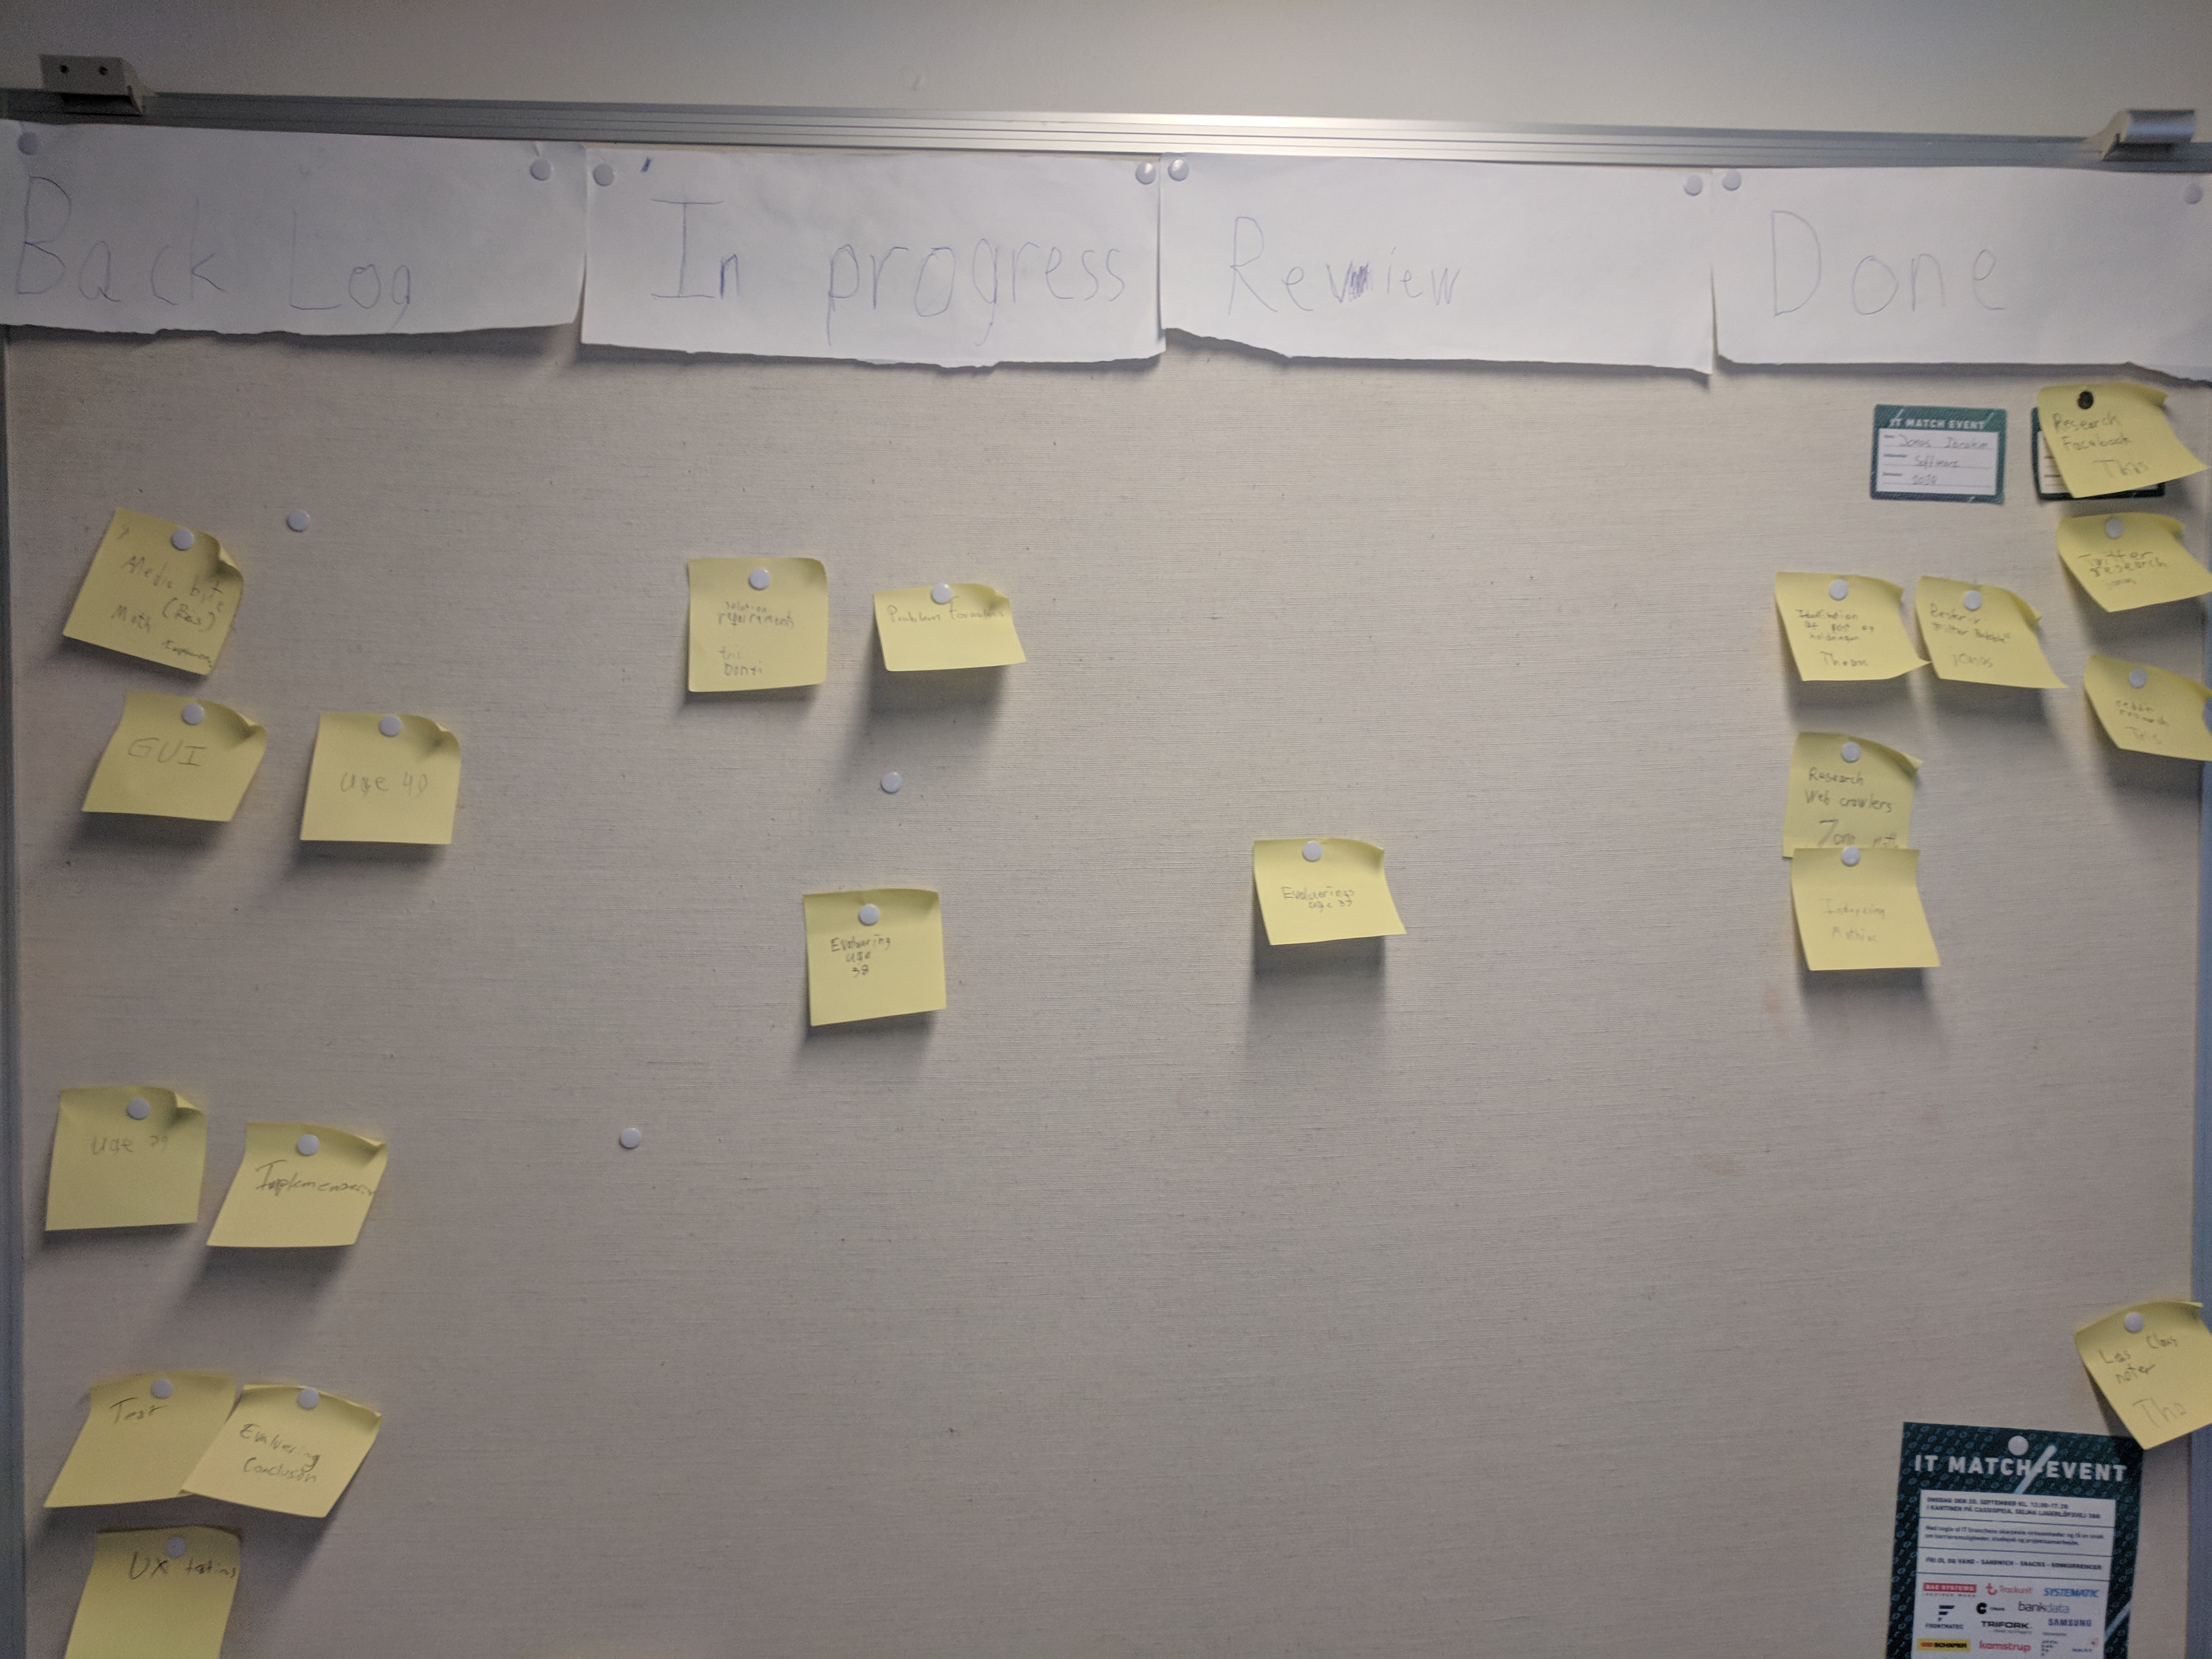
\includegraphics[width =
0.5\textwidth]{figures/Board.jpg}
	\caption{Our board SCRUM element.}
\end{figure}

\subsection*{Reflection}
We had narrowed us down with the social media sites to the ones we thought were
best, therfore we investiated further and found many we had not considered. The
report is progressing but getting updates as we learn new stuff, perhaps we
should have studied some of the topics further to avoid much rewriting in the
analysis part. There are not many gaps in our schedule for project work this
semester, with all the lectures.

We have made some plans to improve the group's structure and workflow. We made a
short description of the final product, but it was mainly for the supervisor to
see, and it will definitely be updated after. We also look forward to seeing how
morning meetings will help with information sharing.

We found that Facebook is a very restrictive media, with its user-data, and does
not part with information easily. We would have to ask for permission to crawl
Facebook, and from the limited amount of crawlers permitted to do so, then it is
unlikely that we will get the chance. Therefore we are starting to look further into
Twitter and Reddit, as a source for user data, on the initial lookup Twitter's
data looks accessible.

\subsection*{Next Week}
During the next week we want to finish the parts of the report in editing, and
get the rest of the analysis into the editing phase. We would also like to get
started on the data gahtering part of the report. Nedxt week will have focus on
indexing the sites crawled, which means we hope that we are able to see the data
we will be working with.





% Facebook is restrictive, besides that we need to ask for permission. So far we
% are thinking of going in a different direction from facebook. We are looking
% into what is available with twitter and reddit. Alot seems to be available at
% twitter.
% 
% Klaus has had a dat 6 group. We have a degree so we can reach out to companies,
% and we seem more professional. We need a to reflect, and evaluate our UI. We can
% look into books and look for what design process we can follow to develop a UI.
% When we test it should not be a mock-up, but if nothing else provide the
% illusion of depth.
% 
% For reflection, we consider adding a chapter for describing the process.
% 
% We edited the filter bubble and Facebook research parts of the report and
% continued work on the webcrawler.
% Finished research on the links from Klaus, and structured an idea for the final
% webagent.
% Begun on the fundamental request builder to fetch information from Twitter.
% 
% 
% Mail Our Progress:
% We have found that Facebook does not seem to be that great for accurate data.
% We have researched on basic crawlers and its seems like we need permission to
% crawl.
% Twitter and Reddit seem like the best options from our current research.
% 
% The agenda for the meeting:
% 1. Web crawlers and limited access to major social hubs, Facebook doesn't want
% people to crawl their sites. While it seems to be limited on Twitter.
% 2. What do you expect from a 7th semester project? Aside from the semester
% description? 3. How should we document our process? Lone said we needed to
% describe this.
% 
% 
% 
% 
% Here are our notes from today's meeting 
% 
% ---------- Current idea
% for the structure of the rapport:
% Intro (problem description)
% 
% Research Social medial Data gathering Web agent?
% 
% Problem Formulation
% 
% GUI design
% 
% Implementation (done by 25. nov)
% 
% Test User tests Evaluation of the UI Other tests?
% 
% Evaluation
% 
% Rapport:
% Introduction seems good.
% Chapter 2 - Should be more distinctly separated, between formal and reflection.
% Be more concrete about everything, less would, should…
% 
% Discussion:
% Twitter has good possibilities, as we can access a lot of data through their
% API, though we can only make a limited amount of calls every 15 min.
% 
% Thoughts on UI:
% What should the user be shown? Can we find enough info to break the bubble We
% will need to briefly describe the process of designing a GUI but we do not need
% to describe the whole process of iterating through the designs.
% 
% Reflections:
% For the process we can describe some of the difficulties of having all the
% different combination of study. As we need to be better to manage our time. We
% should add our experiences with researching facebook, twitter and reddit and why
% we chose what we chose.
